\documentclass[10pt]{article}
\usepackage{graphicx}
\usepackage[margin=1in]{geometry}
\usepackage{titlesec}
\usepackage{multicol}
\usepackage{multirow}
\begin{document}
\begin{center}
\Large{Parcial 2 - Optimizaci\'on}

\Large{Gerardo Andr\'es Ria\~no Brice\~no - 201112388}
\medskip
\hrule
\end{center}

\setlength\parindent{0pt} 

{\bf \Large{Problema 1}}
\medskip

a) La función es no es convexa ni cóncava dado que $F(x)$, matriz Hessiana de $f(x)$ es indefinida. De igual manera para el caso de $-f(x)$, como se muestra a continuación:

\begin{center}
$f(x) = x_1  e^{-x_2}$

$-f(x) = -x_1^{-x_2}$

$x \in R^2 $

$\nabla f(x) = [e^{-x_2}, -x_1e^{-x_2}]$

$F(x) = \left[
{\begin{array}{cc} 
0 & e^{-x_2} \\
e^{-x_2} & x_1e^{-x_2} \\
\end{array}}
\right]$
\end{center}


Dado que $e^{-x_2} > 0$ para todo $x_2$, $det(F(x)) = -e^{-2x_2}$, $det(F(x)) < 0$, por lo tanto $F(x)$ no es semi-definida positiva, y $f(x)$ no es convexa, como $f(x)$ no es convexa, $-f(x)$ no es c\'oncava. 

Para el caso de $-f(x)$, se tiene que:

\begin{center}
$\nabla f(x) = [-e^{-x_2}, x_1e^{-x_2}]$

$F(x) = \left[
{\begin{array}{cc} 
0 & -e^{-x_2} \\
-e^{-x_2} & -x_1e^{-x_2} \\
\end{array}}
\right]$
\end{center} 

De manera similar, $F(x)$ para el caso de $-f(x)$ es indefinida, por lo tanto no es convexa o c\'oncava.

\bigskip

b) Para hallar los puntos que satisfacen la CNPO: 

\begin{center}
$d^T \nabla f(x) \geq 0$

para puntos internos: $\nabla f(x) = 0$
\end{center}


Entonces, sin p\'erdida de generalidad, se hallan los puntos que satisfacen la CNPO para el problema de optmizaci\'on $\min{-f(x)}$. Se tiene que: 

\begin{center}
$\nabla f(x) = [-e^{-x_2}, x_1e^{-x_2}]$
\end{center} 

Para puntos internos, no se satisface la CNPO, i.e. $\nabla f(x) \neq 0$

Ahora bien, es necesario que para $d = (d_1, d_2)$, $d_1 \leq 0, d_2 \geq 0$ dado que $x_1 \geq 0$.

Ahora, se analizan las fronteras de la regi\'on factible, que se muestran en la imagen a continuaci\'on. 


\begin{center}
\begin{figure}[ht!]
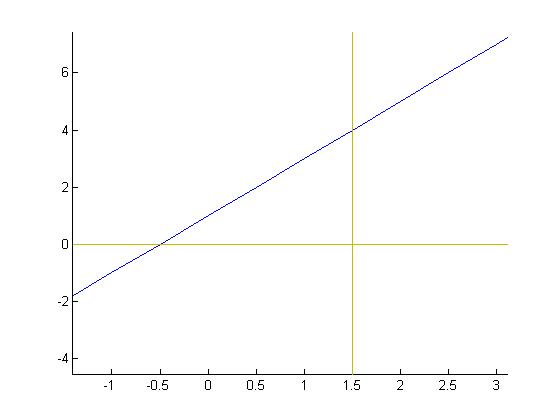
\includegraphics[width=80mm]{matlab/untitled.jpg}
\end{figure}
\end{center}

Primero se revisan las esquinas. En el punto $(0.5, 0)$ no se cumple la CNPO dado que $d_1 > 0$ es factible. En el punto $(1.5 0)$ se satisface la CNPO dado que $d_1 \leq 0$ y $d_2 \geq 0$. Finalmente, en el punto $(1.5, 4)$ no se cumple la CNPO dado que $d_2 < 0$ es factible. Ahora, para la restricci\'on $x_1 \geq 0$ no se cumple que $d_1 \leq 0$ dado que $d_1 > 0$ es factible. Por otro lado, para la restricci\'on, $x_2 \leq 0$ no se cumple la CNPO dado que $d_2 < 0$ es factible. Finalmente, para la restricci\'on $x1 \geq 1 + 2x_2$ no se cumple la CNPO, dado que $d_2 < 0$ y $d_1 > 0$ son factibles.

\bigskip

{\bf \Large{Problema 2}}
\medskip

a) Para definir los costos, \'ultimo d\'igito del c\'odigo igual a 8. Por lo tanto:

\begin{center}
$q=8$, $c_0 = 16$, $c_1 = 8$ y $c_2 = 5$
\end{center}

Para plantear el problema como uno de transporte, se define $x_{ij}$ como el n\'umero de servilletas sucias que se env\'ian a lavar, ya sea con el servicio r\'apido o lento, en el d\'ia i-\'esimo, para ser regresadas el d\'ia j-\'esimo. Asimismo, se define $x_{i0}$ como el n\'umero de servilletas sucias retiradas para un servicio futuro, en el d\'ia i-\'esimo. Entonces, cada d\'ia i-\'esimo representa un origen de servilletas sucias, que deben ser enviadas a lavar y se debe cumplir que: 

\begin{center}
$\sum_{j=1}^{T} x_{ij} + x_{i0} = r_i$, para $i=1,2,...,T$ \\
\end{center}

De manera similar, cada d\'ia j representa un destino de servilletas limpias y $r_j$ servilletas deben recibirse de env\'ios anteriores a la lavander\'ia, del stock, o de una nueva compra. Por lo tanto, se define $x_0i$ como el n\'umero de servilletas compradas el d\'ia j-\'esimo y $x_0k$ el n\'umero de servilletas tomadas del stock. Se tiene entonces que: 

\begin{center}
$\sum_{i=1}^{T} x_{ij}+x_{0i}+x_{0k}$, para $j=1,2,...,T$
\end{center}

Adem\'as debe cumplirse que el sistema es balanceado y que ambas sumatorias descritas anteriormente son iguales y que las servilletas en stock no son m\'as que 200. De esta manera, se puede plantear el problema de la forma t\'ipica de los problemas de transporte.


b) Primero se obtiene la primera soluci\'on b\'asica factible, siguiendo la regla de la esquina noroeste y teniendo en cuenta que ciertos existen viajes imposibles, como los de la fila 4 del tableau, dado que no esposible lavar servilletas del d\'ia 4 para utilizarlas otro d\'ia.

\begin{center}
\begin{figure}[ht!]
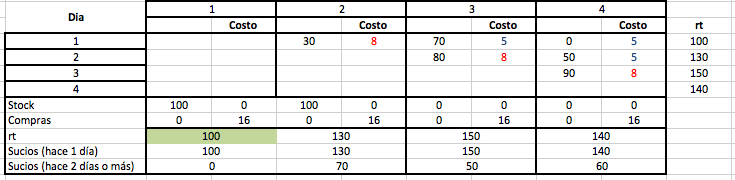
\includegraphics[width=160mm]{im.png}
\end{figure}
\end{center}

\end{document}